% !TEX encoding = UTF-8
% !TEX TS-program = pdflatex
% !TEX root = ../tesi.tex

%**************************************************************
\chapter{Distorsione}
\label{cap:distorsione}
%**************************************************************

\intro{In questo capitolo viene approfondito il fenomeno della distorsione del segnale audio descrivendo alcuni principi teorici fondamentali, analizzando diverse tecniche esistenti e alcune implementazioni digitali presenti sul mercato}\\

%**************************************************************
\section{Introduzione al fenomeno}

Per \textit{distorsione} di un segnale si intende l'\textit{alterazione della forma d'onda} originale, causando la modifica dell'informazione che tale segnale rappresenta. Il fenomeno in questione può risultare indesiderato, come nel caso delle telecomunicazioni in cui se viene prodotto un disturbo nella ricezione del segnale viene alterata l'informazione originariamente trasmessa, oppure desiderato, come nel caso dell'ambito musicale in cui la distorsione viene utilizzata come strumento per la ricerca e il sound design. \\
Il termine distorsione, seppur a livello teorico assuma questo significato, nel contesto musicale viene usato principalmente per riferirsi alla distorsione non lineare e in particolare all'introduzione di nuove componenti frequenziali mediante non linearità\footcite{white-leouie:theaudiodictionary}. \\
La \textit{distorsione lineare} consiste in qualsiasi tipo di alterazione della forma d'onda che non genera nuove frequenze rispetto al segnale originale. Alcuni esempi di questa categoria di distorsione sono l'alterazione dell'ampiezza del segnale (comunemente chiamata regolazione del volume), dipendente dalla frequenza, di un amplificatore e la quantità di attenuazione, sempre dipendente dalla frequenza, da parte di un filtro elettrico\footcite{kleiner:acousticsaudiotech}. \\
Sempre nel contesto musicale esistono diverse fonti di \textit{distorsione non lineare}, alcune delle quali vengono approfondite nella successiva sezione, e la più comune consiste nel \textit{clipping}, ovvero la saturazione di un sistema per la regolazione dell'ampiezza del segnale audio, ottenibile utilizzando circuiti elettrici analogici (per esempio un amplificatore di segnale quando gli viene richiesto di produrre un livello che eccede i suoi limiti di progettazione\footcite{davis-jones:soundreinforcement}) oppure attraverso delle emulazioni digitali.

%**************************************************************
\section{Tecniche di distorsione}

In questa sezione vengono analizzate alcune tecniche di distorsione \textit{non lineari} del segnale audio, tutte implementate nel software Biztortion attraverso appositi algoritmi descritti nel terzo capitolo del presente documento.

\subsection{Clipping}
Il \textit{clipping} consiste in un processo non lineare che produce frequenze non originariamente presenti nel segnale audio. Queste frequenze possono essere armoniche, nel senso che sono multipli interi della frequenza fondamentale del segnale originale, o disarmoniche, ovvero slegate da qualsiasi rapporto con le frequenze del segnale originario. La produzione di armoniche nel segnale è un fenomeno chiamato distorsione armonica, mentre le frequenze spurie possono venire introdotte nel segnale a causa dei comportamenti non lineari nell'elaborazione del segnale utilizzando sia apparecchiature analogiche che algoritmi digitali, a causa del fenomeno della \gls{dimg}. Infatti, ad esempio, suonare un \gls{powerchordg} con la chitarra elettrica attraverso un clipper provoca, oltre all'arricchimento dello spettro sonoro con l'aggiunta delle armoniche del segnale originario, anche un'intermodulazione che produce nuove subarmoniche. \\
Di seguito vengono descritte due diverse modalità di clipping del segnale:
\begin{itemize}
    \item \textbf{Soft clipping}:
        \begin{itemize}
            \item effettua un \textit{appiattimento graduale} dei picchi di un segnale, creando un numero di armoniche più alte che condividono una relazione con il timbro originale;
            \item il soft clipping è ottenibile utilizzando strumentazione analogica ed avviene quando si aumenta un segnale ad una tensione di picco più elevata rispetto a quella che un determinato dispositivo riesce a gestire. Un esempio può essere la distorsione attraverso la saturazione di un amplificatore a \textit{valvole}. Essenzialmente l'aumento del voltaggio spinge le valvole oltre la propria regione di funzionamento lineare, ossia quella regione in cui ad un aumento del voltaggio segue un aumento proporzionale dell'ampiezza del segnale;
            \item questo fenomeno, molto utilizzato per aggiungere carattere al suono delle chitarre elettriche, è ottenibile anche nel mondo digitale implementando un algoritmo che emuli il comportamento della strumentazione analogica. 
        \end{itemize}
    \item \textbf{Hard clipping}:
        \begin{itemize}
            \item effettua un \textit{appiattimento brusco} dei picchi di un segnale, con conseguente maggiore potenza nelle armoniche prodotte dal segnale originario. All'aumentare del clipping, il segnale in ingresso inizia progressivamente ad assomigliare a un'onda quadra con armoniche dispari. Questa viene generalmente descritta come una sonorità più aspra;
            \item l'hard clipping è ottenibile facilmente nel mondo digitale in quanto si verifica quando un segnale viene amplificato oltre 0 \gls{dbfsg} in qualsiasi supporto digitale, come il tipico convertitore analogico/digitale o digitale/analogico. In questi casi, 0 \gls{dbfsg} è il valore più alto in assoluto che il computer può gestire e al di sopra di questo livello le informazioni vengono scartate con il risultato di tagliare la parte superiore della forma d'onda. Ovviamente risulta possibile inoltre implementare un algoritmo che tagli automaticamente ogni informazione del segnale sopra ad una soglia impostata dall'utente;
            \item questo fenomeno risulta ottenibile non solo in digitale ma anche utilizzando strumentazione analogica. Un esempio consiste nell'utilizzo degli \textit{amplificatori a stato solido} che incorporano transistor e/o amplificatori operazionali. Dal punto di vista elettronico, ciò si ottiene solitamente amplificando il segnale fino a un punto in cui viene tagliato dalla limitazione della tensione del binario di alimentazione o clippando il segnale utilizzando i diodi.
        \end{itemize}
\end{itemize}
\begin{figure}[!h] 
    \centering 
    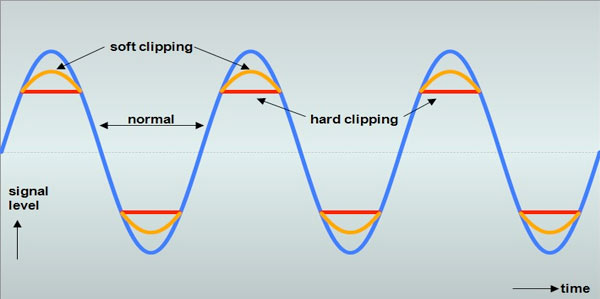
\includegraphics[width=0.8\columnwidth]{immagini/cap2/clipping.jpg}
    \caption{Il fenomeno del Clipping}
\end{figure}

\subsection{Waveshaping}
La tecnica di distorsione del segnale \textit{Waveshaping} viene descritta in modo preciso e puntuale nel libro \textit{The Theory and Technique of Electronic Music}\footcite{puckette:theoryandtechniqueofelectronicmusic} come un passaggio del segnale originale attraverso una funzione non lineare opportunamente scelta. La funzione f(), chiamata \textit{funzione di trasferimento}, distorce la forma d'onda in ingresso in una forma diversa. La nuova forma dipende dalla forma dell'onda in input, dalla funzione di trasferimento e anche, in modo cruciale, dall'ampiezza del segnale in ingresso. Poiché l'ampiezza della forma d'onda in input influenza direttamente la forma della forma d'onda in output (e quindi il timbro), questo dà la possibilità di creare una famiglia di timbri che varia continuamente, semplicemente variando il livello di ingresso della trasformazione. Per questo motivo, è consuetudine includere un controllo di ampiezza iniziale come parte dell'operazione di waveshaping. \\ 
L'ampiezza della forma d'onda in ingresso è chiamata \textit{indice} della forma d'onda. In molte situazioni un indice piccolo porta a una distorsione relativamente piccola (in modo che l'output assomigli molto all'input) e uno più grande dà un timbro più distorto e più ricco. \\
La figura 2.2 mostra un esempio di waveshaping in cui f() equivale a una funzione di clipping. Questo esempio mostra chiaramente come l'indice può influenzare la forma d'onda di output. La funzione di clipping \textbf{(b)} passa il suo input direttamente all'output senza variarlo fintanto che rimane nell'intervallo tra - 0.3 e +0.3. Quindi, quando l'input non supera 0,3 in valore assoluto, l'output è uguale all'input. Tuttavia quando l'input cresce oltre i limiti, l'output viene fatto rimanere entro essi e, all'aumentare dell'ampiezza del segnale, l'effetto di questa azione di clipping diventa progressivamente più importante. Nella figura 2.2 il segnale di input è una sinusoide smorzata \textbf{(a)} e l'output \textbf{(c)} evolve nell'asse x da una forma d'onda quasi quadra all'inizio ad una sinusoide pura alla fine.
\begin{figure}[!h] 
    \centering 
    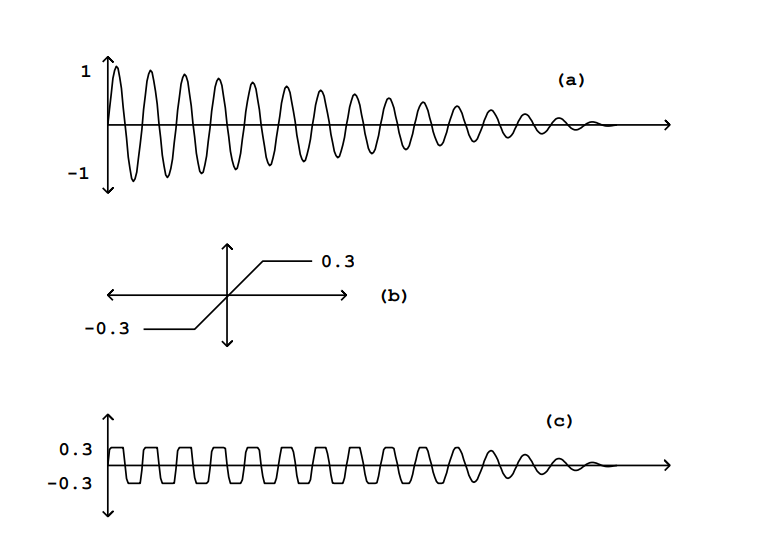
\includegraphics[width=0.8\columnwidth]{immagini/cap2/waveshaper_graph.png}
    \caption{Componenti del Waveshaper}
\end{figure}

\subsection{Bitcrushing}
Il \textit{Bitcrusher} consiste in un processore di segnale che produce distorsione \textit{riducendo la risoluzione dei dati audio digitali}. Gli artefatti introdotti utilizzando questa tecnica possono produrre una sonorità più calda o aspra, a seconda della quantità di degradazione del segnale, andando a simulare il suono prodotto dai vecchi campionatori disponibili all'inizio dell'era digitale. \\
Il bitcrusher utilizza principalmente due metodi per ridurre la fedeltà audio: la riduzione della frequenza di campionamento e la riduzione della profondità di bit.
\begin{itemize}
    \item \textbf{Frequenza di campionamento}: secondo la teoria del campionamento\footcite{burk-polansky-repetto-roberts-rockmore:musicandcomputers}, l'audio digitale è composto da una rapida serie di campioni numerici, acquisiti in modo periodico da un apposito dispositivo chiamato convertitore analogico/digitale, i quali codificano l'ampiezza variabile di una forma d'onda audio. Per una rappresentazione accurata di un segnale audio si necessità di una \textit{frequenza di campionamento} elevata, in quanto maggiore è la frequenza di campionamento, più accurata risulta la forma d'onda. Infatti nel caso in cui il campionamento avvenga ad una frequenza troppo bassa le componenti frequenziali più elevate vengono codificate con troppe poche informazioni e la loro ricostruzione produce degli artefatti. Questo fenomeno, chiamato \textit{aliasing}, avviene nel caso in cui la frequenza di campionamento risulta minore del doppio della frequenza massima del segnale (Teorema del campionamento di Nyquist-Shannon). Sfruttando questo fenomeno il bitcrusher effettua una riduzione graduale, attraverso un apposito parametro, della frequenza di campionamento, introducendo quindi frequenze non armonicamente legate al segnale originale;
    \item \textbf{Profondità di bit}: i singoli campioni nell'audio digitale vengono solitamente registrati come numeri in \textit{virgola mobile} e memorizzati nella memoria digitale utilizzando la \textit{codifica binaria}. In questo modo maggiore è il numero di bit disponibili per rappresentare il livello di ampiezza dei singoli campioni, più accuratamente le forme d'onda vengono campionate. La riduzione della risoluzione effettuata dal bitcrusher riduce intenzionalmente il numero di bit utilizzati per i campioni audio. Man mano che la profondità di bit diminuisce, le forme d'onda diventano più rumorose e si perdono sottili variazioni di volume, riducendo quindi la gamma dinamica. Alla riduzione estrema dei bit a disposizione, le forme d'onda vengono ridotte a delle onde quadre o addirittura a singoli click, aggiungendo quindi molte alte frequenze nello spettro sonoro. 
\end{itemize}
\begin{figure}[!h] 
    \centering 
    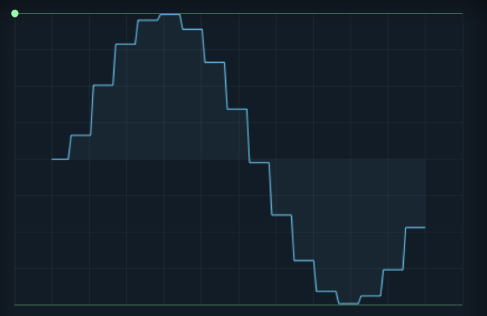
\includegraphics[width=0.8\columnwidth]{immagini/cap2/bitcrusher.png}
    \caption{Riduzione della risoluzione del segnale in un Bitcrusher}
\end{figure}

\subsection{Slew Limiting}
Lo \textit{Slew Limiter} consiste in un processore di segnale audio, solitamente presente come singolo modulo nei sintetizzatori modulari analogici, che permette di livellare un segnale in ingresso in modo che la variazione del livello di tensione non possa superare un certo numero di volt al secondo. Per questo motivo il processore in questione viene solitamente utilizzato come controller di portamento e può essere utilizzato anche come un semplice generatore di inviluppi Attack-Release.\\
Una emulazione digitale di questo particolare processore è implementata nel software Biztortion ed è ispirata al modulo Eurorack \textit{Slew Limiter}\footcite{site:slewlimiter} dell'azienda Befaco, del quale esiste un'implementazione digitale per il software VCV Rack distribuita con \hyperref[cap:licenze-software]{licenza GPL-3.0}. In particolare in questo algoritmo risulta possibile impostare la soglia di velocità massima sopra alla quale essa stessa viene limitata nel tempo sul segnale in uscita, sia nella fase in cui l'onda si muove verso la zona positiva (\textit{Rise}), sia durante la fase in cui l'onda procede nella direzione opposta (\textit{Fall}), andando in questo modo a distorcere la forma d'onda dell'audio.
\begin{figure}[!h] 
    \centering 
    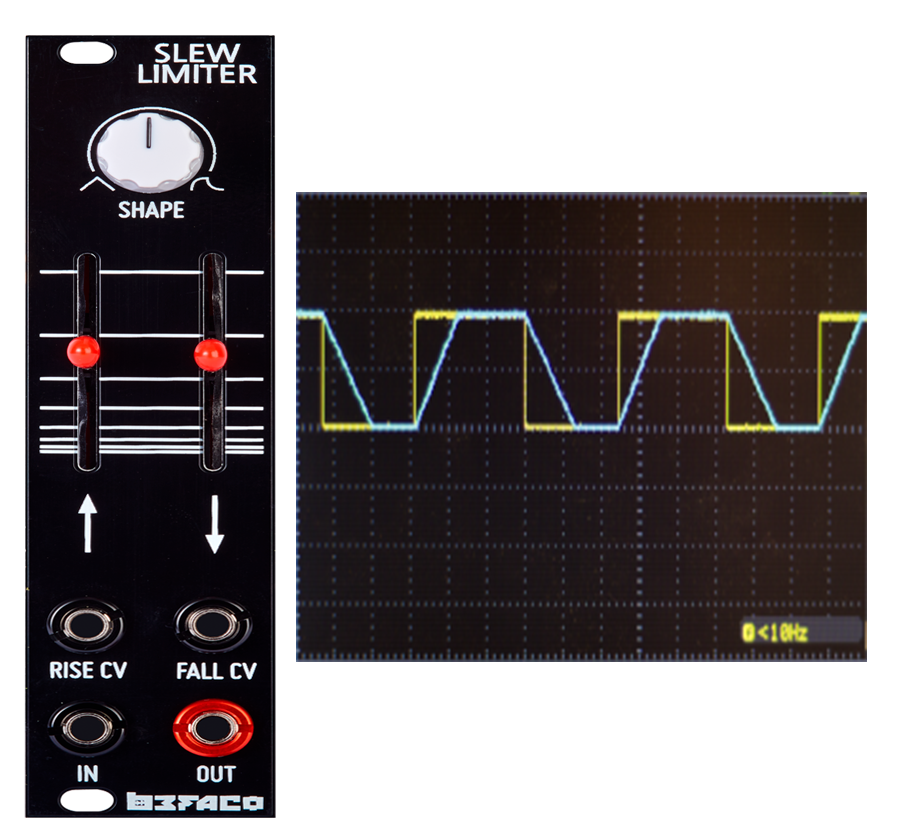
\includegraphics[width=0.8\columnwidth]{immagini/cap2/slew-limiter_Befaco.png}
    \caption{Funzionamento del modulo Slew Limiter dell'azienda Befaco: i segnali in ingresso e uscita sono rispettivamente giallo ed azzurro}
\end{figure}

%**************************************************************
\section{Studio dello stato dell'arte}
In questa sezione viene effettuata un'analisi di alcuni prodotti software presenti sul mercato che offrono diverse tipologie di algoritmi e strumenti utili per la distorsione del segnale audio. \\
Questi prodotti sono stati utilizzati come fonte d'ispirazione per la creazione dell'interfaccia grafica del software \textit{Biztortion}, utili prevalentemente per identificare il layout più funzionale per massimizzare la user experience. Questa ricerca si è rivelata utile inoltre per effettuare un'analisi dei pregi e difetti dei processori di segnale in questione, in modo da poter ricreare nel modo più fedele possibile le funzionalità utili e allo stesso tempo effettuare degli aggiustamenti o aggiunte ad alcuni algoritmi nel software sopraccitato.

\subsection*{Izotope Trash 2}
\noindent \textit{Izotope Trash 2}\footcite{site:trash2} consiste in un processore di segnale audio digitale, disponibile come \gls{pluging} audio in diversi formati, che consente una trasformazione sonora complessa grazie alla presenza di un elevato numero di moduli che offrono diverse funzionalità.
%\clearpage
\begin{figure}[!h] 
    \centering 
    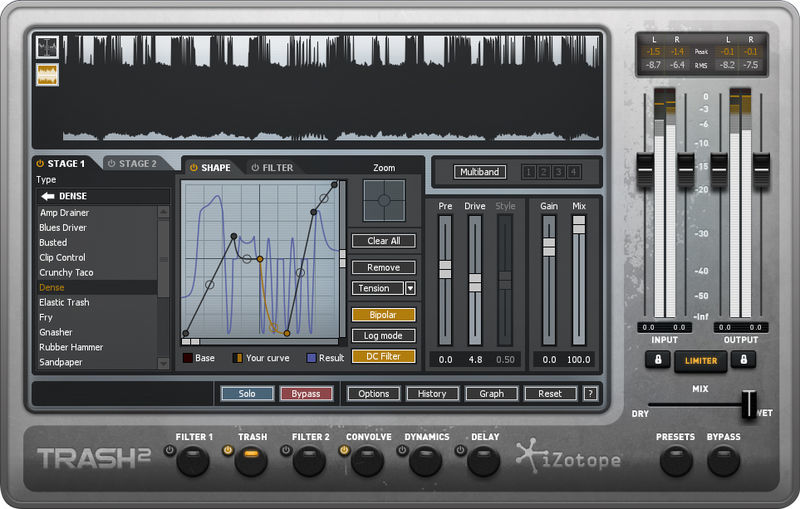
\includegraphics[width=0.8\columnwidth]{immagini/cap2/trash2.jpg}
    \caption{Izotope Trash 2}
\end{figure} \\
I moduli offerti dal software sono i seguenti:
\begin{itemize}
    \item \textbf{Pre/Post-filtering}: i moduli per il filtraggio del segnale consentono di modellare lo spettro sonoro utilizzando fino a 6 filtri, i quali possono essere configurati con oltre 20 modelli differenti. Sono inoltre utilizzabili degli \gls{lfog}, inviluppi e il \gls{sidechaing} per la modulazione dei parametri;
    \item \textbf{Trash}: il modulo in questione consente la distorsione del segnale utilizzando oltre 60 funzioni di trasferimento per effettuare waveshaping in due stadi, con la possibilità di applicare l'effetto a tutto lo spettro o fino a 4 bande di frequenze differenti;
    \item \textbf{Convolve}: attraverso il modulo per la convoluzione del segnale Trash 2 consente una simulazione realistica di diversi altoparlanti ed acustiche, permettendo di posizionare completamente l'audio in un altro luogo o oggetto;
    \item \textbf{Dynamics}: consente la compressione multibanda del segnale utilizzando fino a 4 bande di frequenze differenti;
    \item \textbf{Delay}: consente l'aggiunta dell'effetto Echo offrendo fino a 6 algoritmi diversi.
\end{itemize}

\subsection*{Kilohearts Toolbox}
\noindent \textit{Kilohearts Toolbox}\footcite{site:toolbox} consiste in un pacchetto, del quale esistono diverse versioni in base al budget che si vuole investire nel suo acquisto, che offre vari strumenti che fanno parte dell'ecosistema Kilohearts. In questo pacchetto sono compresi diversi \gls{pluging} audio, utilizzabili singolarmente all'interno della \gls{dawg} desiderata, e l'host di effetti modulari gratuito, Snap Heap, per poter combinare i singoli \gls{pluging} in rack di effetti seriali e/o paralleli. \\
\begin{figure}[!h] 
    \centering 
    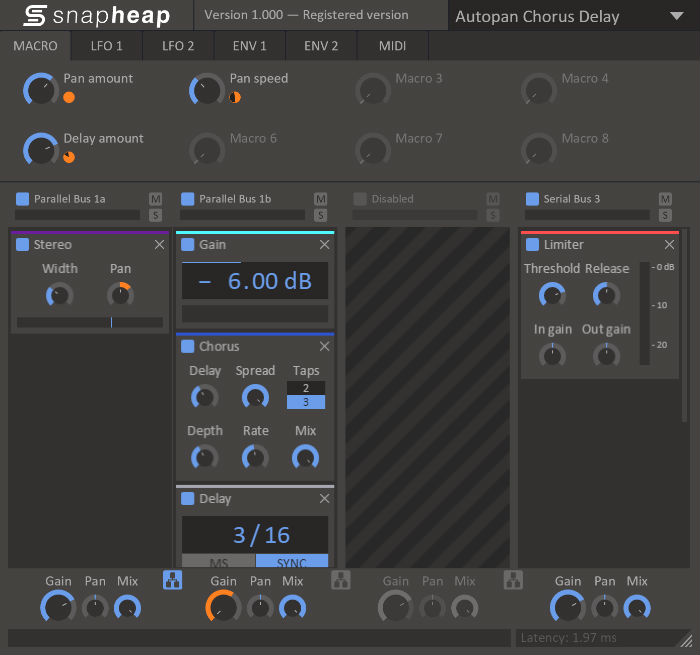
\includegraphics[width=0.8\columnwidth]{immagini/cap2/kilohearts.jpg}
    \caption{Kilohearts Snap Heap}
\end{figure} \\
Tra l'elevato numero di effetti presenti nel pacchetto in questione sono compresi i seguenti \gls{pluging} che effettuano la distorsione del segnale:
\begin{itemize}
    \item \textbf{Distortion}: consiste in un processore di segnale in cui è possibile utilizzare 5 diversi algoritmi, i quali utilizzano diverse combinazioni di waveshaping e filtri, per la distorsione dell'audio in ingresso. Risulta inoltre possibile aggiungere un DC offset al segnale prima del processing e, utilizzando un apposito potenziometro, differenziare l'offset stesso tra i due canali sinistro e destro, in modo da creare dei sottili ampliamenti della stereofonia;
    \item \textbf{Bitcrush}: permette di simulare l'audio come se fosse riprodotto utilizzando un campionatore di bassa qualità, con frequenza di campionamento e profondità di bit limitate. Questo processore di segnale consente inoltre l'aggiunta di rumore in modo effettuare del \gls{ditheringg} per ridurre il rumore causato dalla quantizzazione, oltre all'utilizzo di appositi filtri per la diminuzione dell'aliasing causato dalla riduzione della qualità del campionamento (sia ad alte che basse frequenze);
    \item \textbf{Phase Distortion}: consiste in un processore audio che consente al segnale di modulare la fase di se stesso, risultando sostanzialmente in qualcosa di simile al feedback FM. Questo effetto infatti non modifica l'ampiezza del segnale, come effettuano invece i distorsori tradizionali, ma trasforma la fase di singole armoniche usando l'input stesso come modulante. Poichè l'input influenza direttamente l'algoritmo per la produzione del segnale in uscita, l'effetto risultante è sempre originale e non può suonare uguale in due moduli diversi.
\end{itemize}

% TODO : aggiungo paragrafo con descrizione Fabfilter Saturn

\subsection*{Fabfilter Saturn 2}
\noindent \textit{Fabfilter Saturn 2}\footcite{site:saturn2} consiste in un processore di segnale audio digitale, disponibile come \gls{pluging} audio in diversi formati, che offre una vasta gamma di algoritmi di distorsione ispirati al mondo analogico vintage degli amplificatori a valvole e dei nastri magnetici. Sono inoltre presenti diversi algoritmi basati su differenti tecniche di distorsione come il bitcrushing o la granularizzazione del segnale. 
\begin{figure}[!h] 
    \centering 
    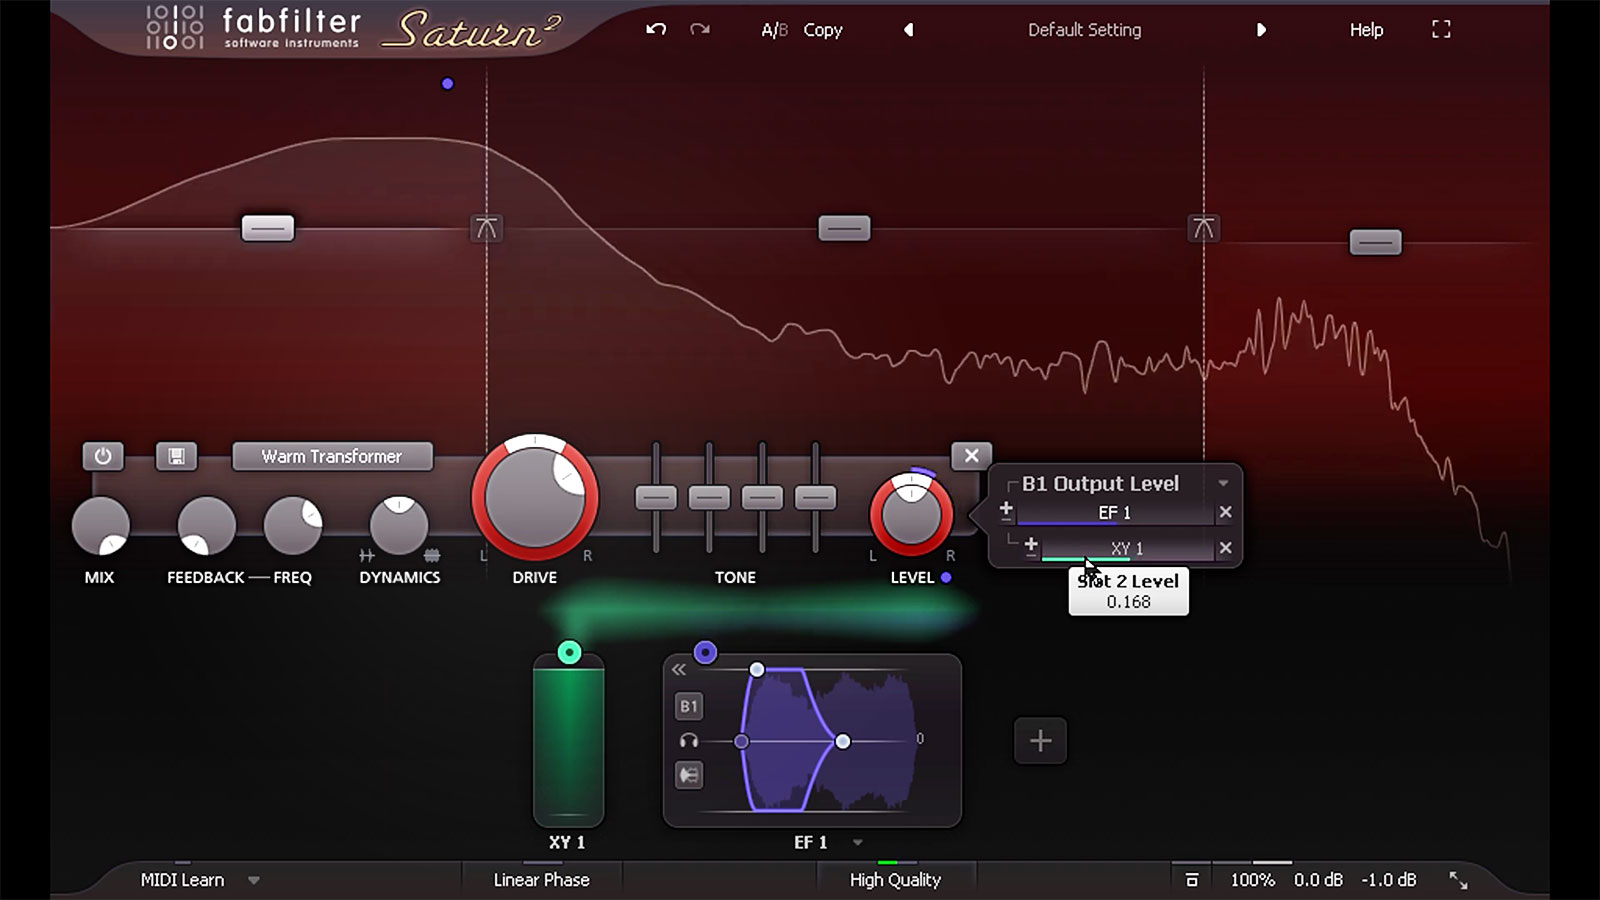
\includegraphics[width=0.8\columnwidth]{immagini/cap2/saturn2.jpg}
    \caption{Fabfilter Saturn 2}
\end{figure} \\
Le funzionalità salienti del software sono le seguenti:
\begin{itemize}
    \item \textbf{Display multibanda interattivo}: il display interattivo consente di creare e selezionare direttamente le bande di frequenza e, allo stesso tempo, è un analizzatore di frequenza in tempo reale, permettendo di visualizzare il segnale in uscita e rendendo facile decidere dove impostare le frequenze di crossover della banda;
    \item \textbf{Controlli delle bande}: i controlli delle bande controllano le impostazioni delle bande selezionate nel display. Per ogni banda, è possibile regolare separatamente il tipo di distorsione, il drive, le impostazioni di feedback, le dinamiche, il tono, il livello e le impostazioni di mix;
    \item \textbf{Sezione di modulazione}: la sezione di modulazione, presente nella parte inferiore dell'interfaccia mostra tutte le sorgenti disponibili per la modulazione dei parametri, ovvero  \gls{lfog}, envelope generator (EG), envelope follower (EF), controller MIDI e XY;
    \item \textbf{Fase lineare}: quando la modalità "Linear Phase" è abilitata, sia il filtro crossover multibanda che l'oversampling interno, attivabile attraverso la modalità "High Quality", vengono eseguiti utilizzando un filtraggio a fase lineare.
\end{itemize}